% !TEX root = main.tex
\chapter{序論}
\section{研究背景}
\subsection{半導体レーザー}
\subsubsection{半導体レーザーの現状}
半導体レーザーが実現されたのは1962年のことである 。キャリアと光の閉じ込めを能率よくできるようにした2重ヘテロ構造が用いられ流ようになり実用化・発展を遂げた。光通信、光ディスク用発光デバイスの核をなす技術である。他のレーザーにと比較しても小型・軽量、大量生産可能、熱や振動(安定性)に強い、高い発振波長選択性などが主な理由である。近年では半導体からピコ秒程度の超短光パルスを発生させる技術も研究が盛んに行われており、産業への応用が期待されている。
%[利得スイッチングsds生物発光yokoyamaさん,ここではGSにこだわらなくてもいいか][psパルスを使った産業]
\subsubsection{超短パルス発生}
ピコ秒オーダーの超短パルスを発生する技術は長距離光ファーバー伝送\cite{ref_hasegawa}に加えて、精密レーザー加工\cite{ref_chichkov} や多光子励起顕微鏡を用いたバイオイメージング[]など、応用の幅が広がってきている技術である。

半導体レーザーを用いた短パルス発生の代表的な方法としては利得スイッチングとモード同期法がある。利得スイッチング\cite{h_ito}は注入電流を変調する直接変調を用いた方法である。デバイスにナノ秒程度の電流パルスを注入すると励起パルスよりも短い、数十psの光パルスが得られるというものである。半導体内の光強度が大きくなると誘導放出によって利得が急激に減少するためである。特徴としては複雑な構造を必要とせずずべての半導体レーザーで実現可能な技術であるという点である。

一方のモード同期法はサブps程度の超短パルスを得ることができる技術である。外部共振器あるいは共振器内に過飽和吸収体を挿入するなど付加的な構造が必要となる。

本研究では比較的容易に実現できる利得スイッチングに注目する。
\begin{comment}
 半導体から短パルスを発生させる方法として従来行われてきた方法が主に3つある。モード同期法、Qスイッチ法、利得スイッチ法である。モード同期法は個体レーザーでも用いられておりフーリエ限界に近いパルス幅を生成できる反面パルスの繰り返し周期が固定されてしまうという特徴を持つ。一方Qスイッチング法は過飽和吸収帯を用いるなどしてQ値を瞬間的に増大させることで高エネルギーの光パルスを得ることができる。利得スイッチングは電流を変調する直接変調の一種であり、複雑な構造を必要とせず、全ての半導体レーザーで実現が可能な技術である。レーザー加工などの技術的応用においては繰り返し可変であることや様々な種類の光源を試すことができるという利点があるため、??本研究では利得スイッチング法に着目した。
\end{comment}


\subsubsection{利得スイッチング法}
半導体レーザーのデバイス中のキャリア密度と光子密度の時間変化の振る舞いは以下のレート方程式で記述される。nは量子井戸1層あたりのキャリア密度、sは全活性層の光子密度を表す。式(\ref{eq:late_eq_1})はnの時間変化を記述している。右辺第1項は外部から注入されるポンプキャリア、第2項は誘導放出、第3項は自然放出を表す。式(\ref{eq:late_eq_2})は光子の時間変化を記述しており、第1項は誘導放出による増幅、第2項は光子寿命による減衰(共振器寿命)、第3項は自然放出光による増幅を表す。
\begin{eqnarray}
\dfrac{dn}{dt}&=&n_{\rm{pump}}\zeta(t)-\dfrac{\Gamma}{m}\nu_{\rm{g}}g(n)\dfrac{s}{1+\epsilon s}-\dfrac{n}{\tau_{r}}\\
\label{eq:late_eq_1}
\dfrac{ds}{dt}&=&\Gamma\nu_{g}g(n)\dfrac{s}{1+\epsilon s}-\dfrac{s}{\tau_{p}}+m\beta\dfrac{n}{\tau_{r}}
\label{eq:late_eq_2}
\end{eqnarray}
\begin{eqnarray*}
&n& : 量子井戸1層あたりのキャリア密度 [m^{-3}]\\
&s& : 活性層全体の光子密度[m^{-3}]\\
&n_{\rm{pump}}& : 励起キャリア密度 \\
&\zeta(t)& : 規格化された励起パルスの時間変化\\
&\Gamma & : 光閉じ込め係数\\
&m& : 量子井戸数\\
&\nu_{g}& : 群速度[m/s]=c/n_{eq}?\\
&g(n)& : 利得[cm^{-1}]\\
&\epsilon & : 利得圧縮係数?\\
&\tau_{r}& : キャリア寿命[s^{-1}]\\
&\tau_{p}& : 光子寿命 [s^{-1}]\\
&\beta& : 自然放出光係数\\
\end{eqnarray*}


上式のようなレート方程式を基に短い励起パルスを印可した時の発光および利得の時間変化についてシミュレーションを行った結果を図\ref{fig:fig_1_1_GS_ito}aに示す。赤線が光励起によるインパルス励起の様子、青線が電流注入による数ns秒パルス励起の様子である。青線に注目すると図\ref{fig:fig_1_1_GS_ito}a上段での励起パルスよりも短い、数十ps光パルスが出てくることがわかる。さらに1つ目のパルスの後は緩和振動が起きている。これが典型的な利得スイッチング動作である。また下段には利得の時間変化が示されている。励起が始まると同時に利得が増えていき、反転分布となると今度は誘導放出によって一気にキャリアが放出される様子がわかる。


次に過去に行われた研究について述べる。利得スイッチングによる短パルス化は長年行われてきており、図\ref{fig:fig_1_1_GS_ito}bに過去40年間に報告されたパルス幅がプロットされている。赤がは光励起、青は電流注入を表している。青を見てみると最短でも5ps程度である。
\begin{figure}[h]
	\centering
	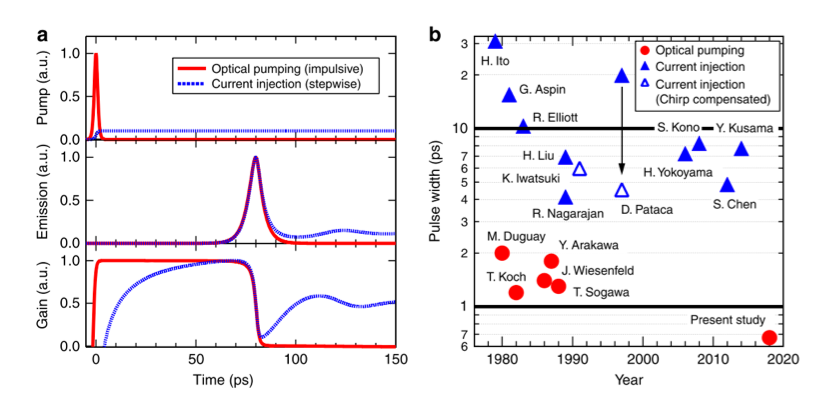
\includegraphics[width=15cm]{figure/fig_1_1_GS_ito.png}
	\caption{a 利得スイッチングのメカニズム, b過去の研究におけるパルス幅\cite{ref_t_ito}}
	\label{fig:fig_1_1_GS_ito}
\end{figure}

\subsubsection{利得スイッチング光パルスの短パルス化}

ではどのような半導体ならば短いパルスが出てくるのかという疑問に達しますがこのような先行研究がなされています。この2つの連立方程式はそれぞれキャリアとフォトンの時間変位を記述するレート方程式です。先ほどのシミュレーションも同等の式に従って計算されたものです。この研究の中ではキャリアのフォトンへの変換効率に寄与するgというファクターが高いほど発生パルスが短くなるということが示唆され、実験的に示されました。

\begin{figure}[h]
	\centering
	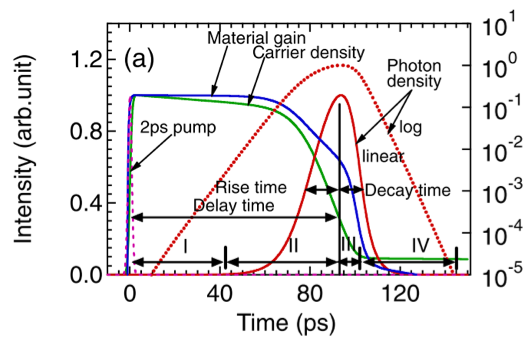
\includegraphics[width=15cm]{figure/fig_1_1_GS_pulse.png}
	\caption{パルス生成中のキャリア密度、光子密度、利得gの時間変化\cite{ref_1_1_GS}}
	\label{fig:fig_1_1_GS_pulse}
\end{figure}

\subsection{InGaAs高利得材料}

\begin{figure}[h]
	\centering
	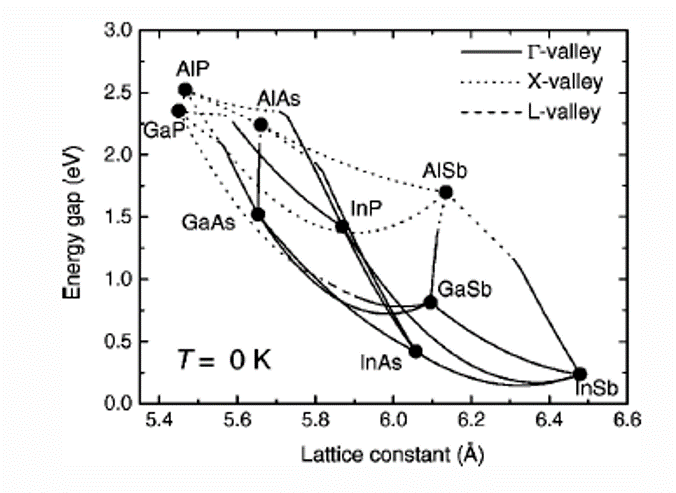
\includegraphics[width=15cm]{figure/fig_1_1_lattice_constance.png}
	\caption{格子定数}
	\label{fig:fig_latice_constancce}
\end{figure}

\begin{figure}[h]
	\centering
	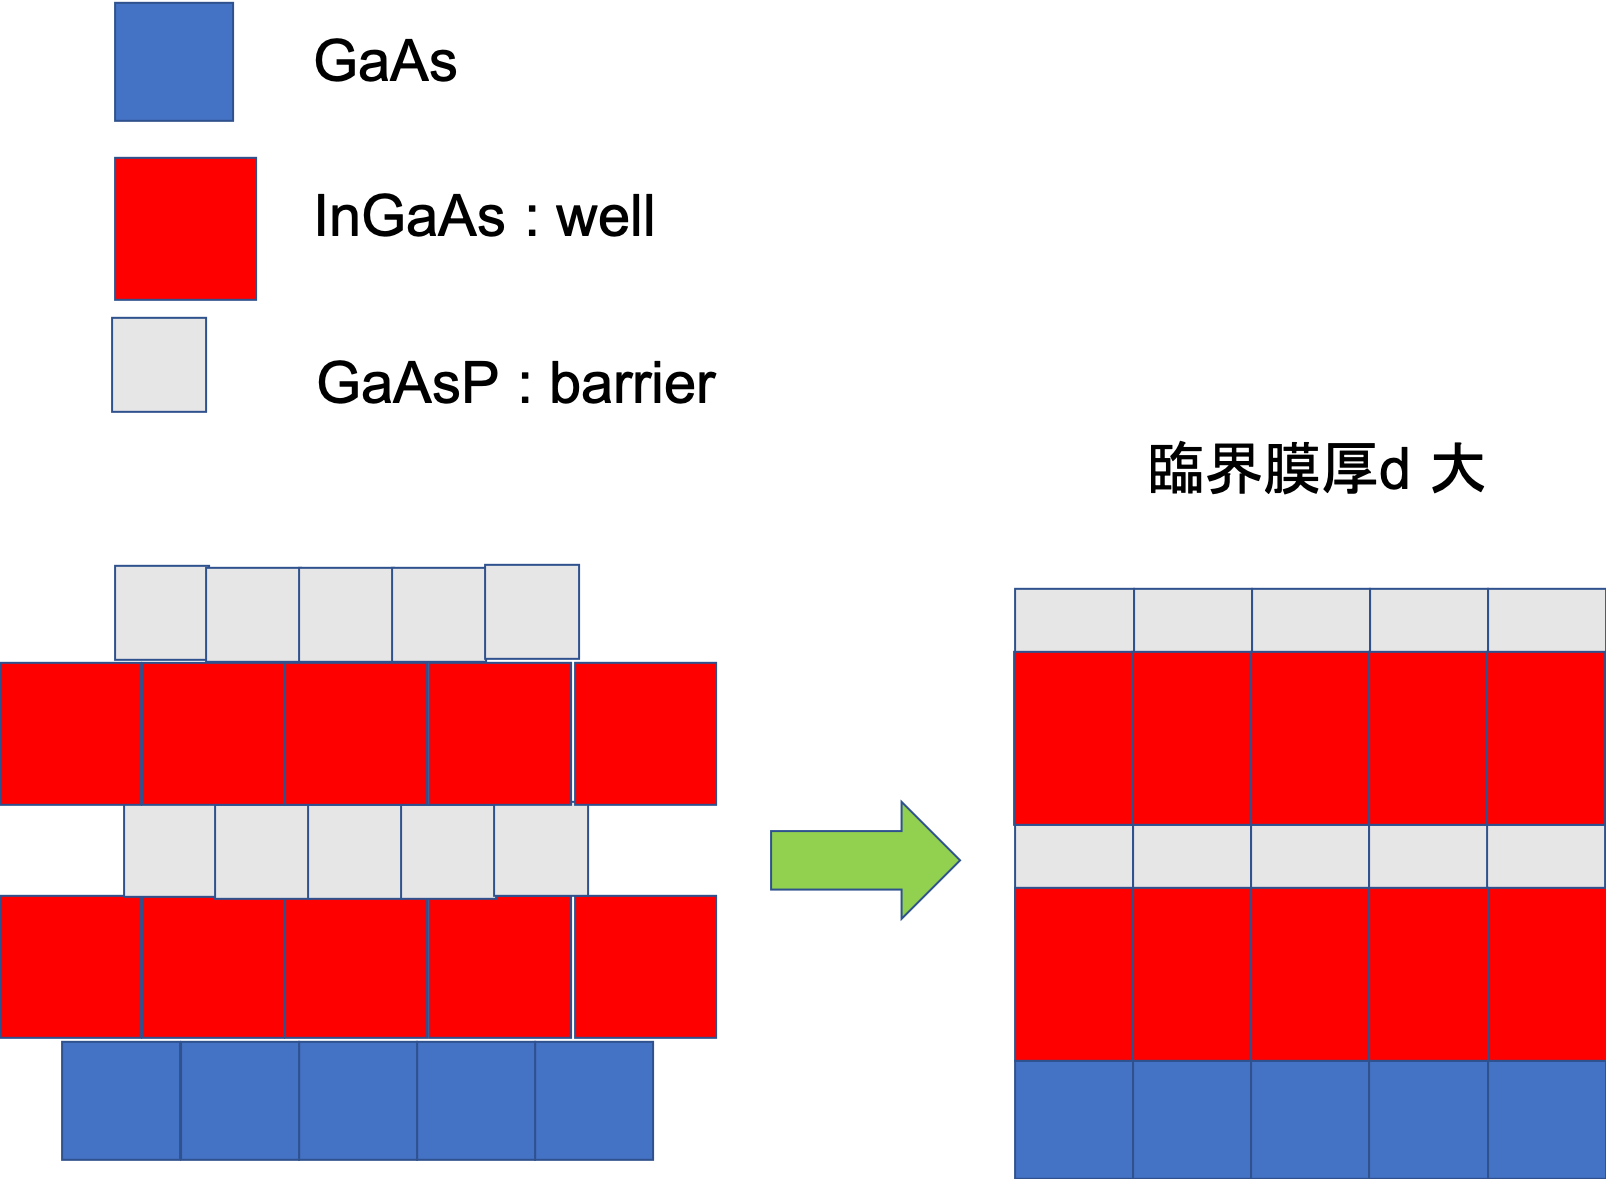
\includegraphics[width=15cm]{figure/fig_1_1_lattice_strain.png}
	\caption{歪み補償}
	\label{fig:fig_1_1_GS_lattice_strain}
\end{figure}
InGaAs
\clearpage
\section{本研究の目的}
電流注入により短いパルスを達成すること?
新しい構造を作ったからそれを図ること?
